\documentclass[11pt]{article}
\usepackage{url}
\usepackage{listings}
\usepackage{tikz}
\usepackage{fontspec}
\usepackage{enumitem}
\setmainfont{Latin Modern Roman}
\setmonofont{Cousine}[Scale=MatchLowercase]
\usetikzlibrary{arrows,automata,shapes}
\tikzstyle{block} = [rectangle, draw, fill=blue!20, 
    text width=5em, text centered, rounded corners, minimum height=2em]
\tikzstyle{bt} = [rectangle, draw, fill=blue!20, 
    text width=1em, text centered, rounded corners, minimum height=2em]

\newtheorem{defn}{Definition}
\newtheorem{crit}{Criterion}
\newcommand{\true}{\mbox{\sf true}}
\newcommand{\false}{\mbox{\sf false}}

\newcommand{\handout}[5]{
  \noindent
  \begin{center}
  \framebox{
    \vbox{
      \hbox to 5.78in { {\bf Software Testing, Quality Assurance and Maintenance } \hfill #2 }
      \vspace{4mm}
      \hbox to 5.78in { {\Large \hfill #5  \hfill} }
      \vspace{2mm}
      \hbox to 5.78in { {\em #3 \hfill #4} }
    }
  }
  \end{center}
  \vspace*{4mm}
}

\newcommand{\lecture}[4]{\handout{#1}{#2}{#3}{#4}{Lecture #1}}
\topmargin 0pt
\advance \topmargin by -\headheight
\advance \topmargin by -\headsep
\textheight 8.9in
\oddsidemargin 0pt
\evensidemargin \oddsidemargin
\marginparwidth 0.5in
\textwidth 6.5in

\parindent 0in
\parskip 1.5ex
%\renewcommand{\baselinestretch}{1.25}

\usepackage[listings]{tcolorbox}
\newtcbinputlisting{\codelisting}[3][]{
    extrude left by=1em,
    extrude right by=2em,
    listing file={#3},
    fonttitle=\bfseries,
    listing options={basicstyle=\ttfamily\footnotesize,numbers=left,language=Java,#1},
    listing only,
    hbox,
}
\lstset{ %
language=Java,
basicstyle=\ttfamily,commentstyle=\scriptsize\itshape,showstringspaces=false,breaklines=true,numbers=left}

\definecolor{gray}{rgb}{0.4,0.4,0.4}
\definecolor{darkblue}{rgb}{0.0,0.0,0.6}
\definecolor{cyan}{rgb}{0.0,0.6,0.6}

\lstdefinelanguage{XML}
{
  morestring=[b]",
  morestring=[s]{>}{<},
  morecomment=[s]{<?}{?>},
  stringstyle=\color{black},
  identifierstyle=\color{darkblue},
  keywordstyle=\color{cyan},
  morekeywords={xmlns,version,type}% list your attributes here
}


\begin{document}

\lecture{32 --- March 24, 2017}{Winter 2017}{Patrick Lam}{version 2}

We've seen two tools so far: PMD and jshint. These tools both operate on
Abstract Syntax Trees and ensure relatively shallow program properties. Out of the
box, PMD guarantees generic properties (but we also talked about writing our own
checkers). 

jshint, PMD, and other tools (like FindBugs, below) enforce generic
rules that all programs should satisfy. You can read a
comparison of different tools in this paper:
\begin{center}
  \url{www.cs.umd.edu/~jfoster/papers/issre04.pdf}
\end{center}

\paragraph{FindBugs.} This tool is somewhat deeper than PMD. FindBugs is an 
open-source static \emph{bytecode} analyzer for Java out of the
University of Maryland.  A key difference is that it performs static
analysis at Java bytecode level rather than AST level. It's therefore
harder to write FindBugs rules.
\begin{center}
  \url{findbugs.sourceforge.net}
\end{center}
FindBugs finds bug patterns like:
\begin{itemize}[noitemsep]
    \item off-by-one;
    \item null pointer dereference;
    \item ignored {\tt read()} return value;
    \item ignored return value (immutable classes);
    \item uninitialized read in constructor;
    \item and more\ldots
\end{itemize}
Such patterns are typically easier to evaluate at bytecode level because the
variability of the AST has been compiled away.

\paragraph{False positives.}
FindBugs, like all static analysis tools, gives some false positives.
(The course project has a question about false positives.) In general, they
occur because the analysis tool is not powerful enough. Because of the
halting problem, there can be no all-powerful tool.

Consider this case:
\begin{lstlisting}
  try { socket.close(); }
  catch (Exception ignore) {}

  try { reader.close(); }
  catch (Exception ignore) {}
\end{lstlisting}
FindBugs, of course, declares ``this method might ignore an exception'', but it's fine in
this case, since there's nothing that the program needs to do about failed close actions.

\newpage
Here are some techniques to help avoid false positives:
\begin{center}
  \url{patricklam.ca/papers/14.msr.saa.pdf}
\end{center}

\section*{Beyond hard-coded rules}

\paragraph{Inferring specifications: Coverity Static Analyzer.} 
This industrial-strength tool (statically) identifies bugs in C/C++,
Java, and C\# codebases. It claims to scale to ``hundreds of users,
thousands of defects, and millions of lines of code in a single
analysis.'' It does so by inferring must-beliefs and may-beliefs from
the code base, as we've discussed in Lecture 22. Coverity does a lot
of work to keep the false positive rate low. Your project reproduces some 
of the key technology behind Coverity.

Coverity is a commercial product which can find many bugs in large
(millions of lines) programs; it is therefore a leading company in
building bug detection tools. Clients (900+) include organizations
such as Blackberry, Yahoo, Mozilla, MySQL, McAfee, ECI Telecom,
Samsung, Siemens, Synopsys, NetApp, Akamai, etc. These include domains
including EDA, storage, security, networking, government (NASA, JPL),
embedded systems, business applications, operating systems, and open
source software.  We have access to Coverity for this course, but
there's also a free trial:
\begin{center}
  \url{http://softwareintegrity.coverity.com/FreeTrialWebSite.html}
\end{center}


\subsection*{Developer-provided specifications}
A number of research-quality tools aim to enforce developer-provided specifications.
Developers should be aware of how their software works. Specification languages
enable developers to express this knowledge in a machine-readable way and tools
can enforce that the software satisfies its specification. We'll discuss some 
specification-based tools below.

\paragraph{Korat (University of Illinois).}
Key Idea: Generate Java objects from a representation invariant specification
written as a Java method.

For instance, here's a binary tree: 

\begin{center}
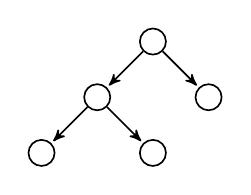
\begin{tikzpicture}[->,>=stealth',shorten >=1pt,auto,node distance=1cm,
                    semithick,initial text=]

  \node[circle,draw]   (0)                    {};
  \node[circle,draw]   (1) [below left of=0]  {};
  \node[circle,draw]   (2) [below right of=0] {};
  \node[circle,draw]   (3) [below left of=1] {};
  \node[circle,draw]   (4) [below right of=1] {};
  
  \path (0) edge              node {} (1)
        (0) edge              node {} (2)
        (1) edge              node {} (3)
        (1) edge              node {} (4);
\end{tikzpicture} 
\end{center}

One characteristic of a binary tree:
\begin{itemize}
\item left \& right pointers don't refer to same node.
\end{itemize}

\newpage
We can express that characteristic in Java as follows:
{\small \begin{lstlisting}[language=Java]
boolean repOk() {
  if (root == null) return size == 0; 	   	      // empty tree has size 0
  Set visited = new HashSet(); visited.add(root);
  List workList = new LinkedList(); workList.add(root);
  while (!workList.isEmpty()) {
    Node current = (Node)workList.removeFirst();
    if (current.left != null) {
      if (!visited.add(current.left)) return false; // acyclicity
      workList.add(current.left);
    }
    if (current.right != null) {
      if (!visited.add(current.right)) return false; // acyclicity
      workList.add(current.right);
    }
  }
  if (visited.size() != size) return false; 	     // consistency of size
  return true;
}
\end{lstlisting}
}

Korat then generates all distinct (``non-isomorphic'') trees, 
    up to a given size (say 3).
It uses these trees as inputs for testing 
    the {\tt add()} method of the tree (or for any other methods.)

    \begin{center}
    \url{korat.sourceforge.net/index.html}
  \end{center}


\end{document}
